\section{Clasificación}

\subsection{Metodología}

\begin{figure}[t]
    \center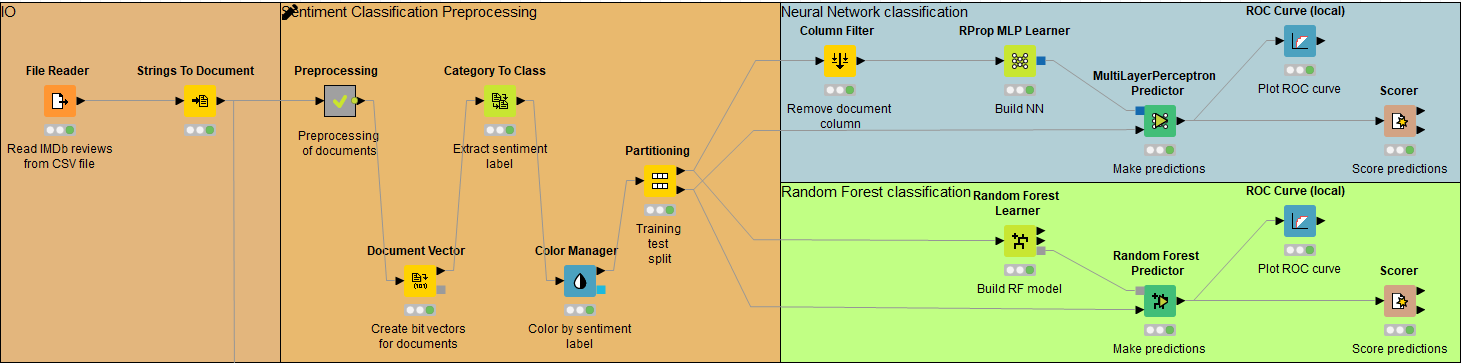
\includegraphics[width=.95\linewidth]{img/classification/workflow.png}
    \caption{Workflow de la clasificación de sentimientos.}
\end{figure}

\begin{figure}[t]
    \center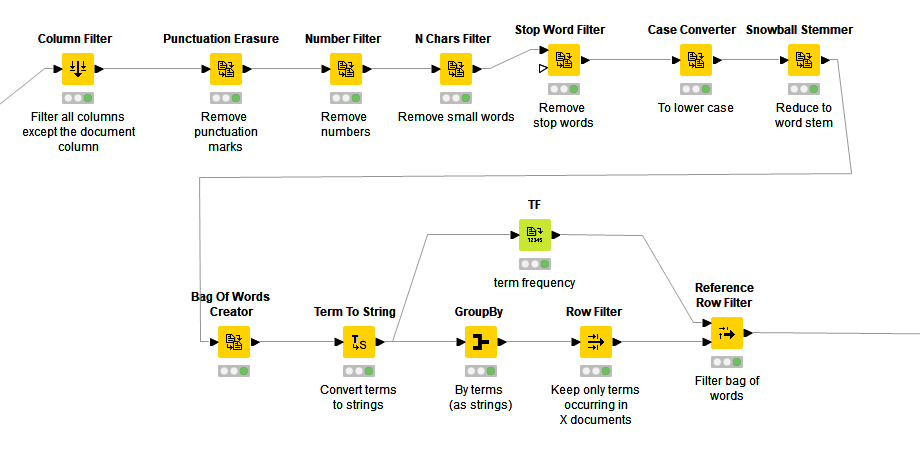
\includegraphics[width=.95\linewidth]{img/classification/preprocessing.png}
    \caption{Preprocesamiento de los documentos.}
\end{figure}

% ----------------

\subsection{Resultados}

\begin{figure}[t]
    \center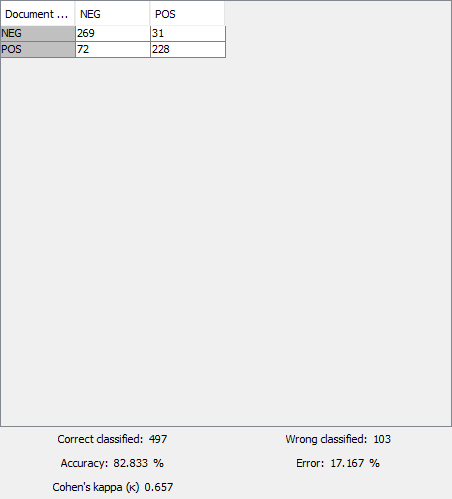
\includegraphics[width=.95\linewidth]{img/classification/cmNN.png}
    \caption{Matriz de confusión con Redes Neuronales.}
\end{figure}

\begin{figure}[t]
    \center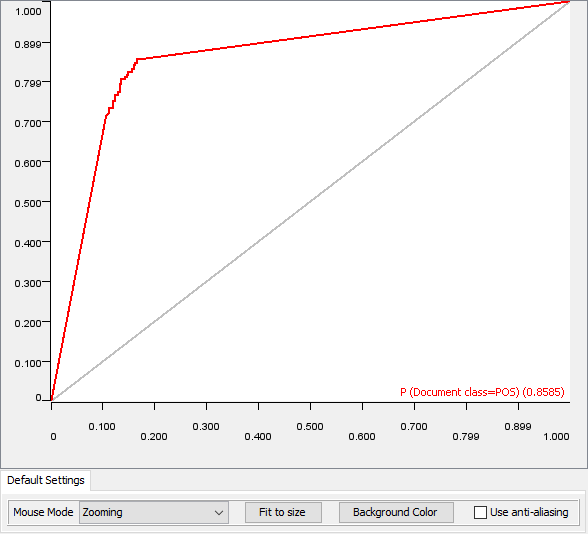
\includegraphics[width=.95\linewidth]{img/classification/rocNN.png}
    \caption{Curva ROC con Redes Neuronales.}
\end{figure}

\begin{figure}[t]
    \center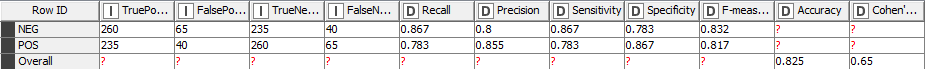
\includegraphics[width=.95\linewidth]{img/classification/scoresNN.png}
    \caption{Medidas estadísticas con Redes Neuronales.}
\end{figure}

% ----------------

\begin{figure}[t]
    \center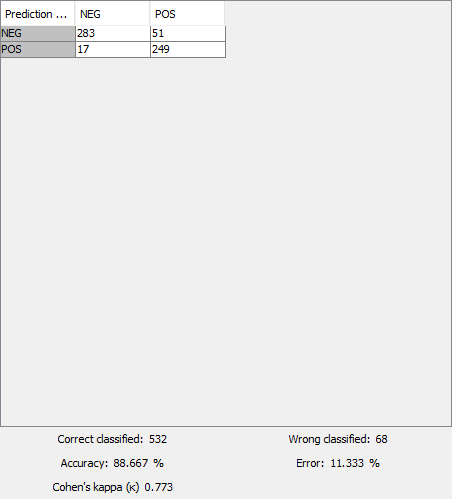
\includegraphics[width=.95\linewidth]{img/classification/cmRF.png}
    \caption{Matriz de confusión con Redes Neuronales.}
\end{figure}

\begin{figure}[t]
    \center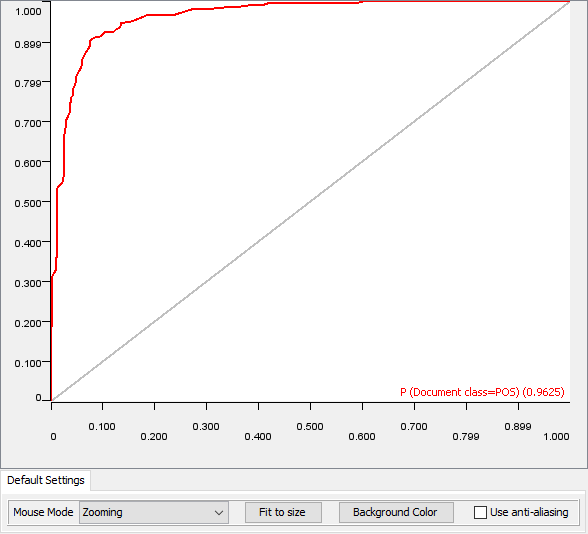
\includegraphics[width=.95\linewidth]{img/classification/rocRF.png}
    \caption{Curva ROC con Random Forest.}
\end{figure}


\begin{figure}[t]
    \center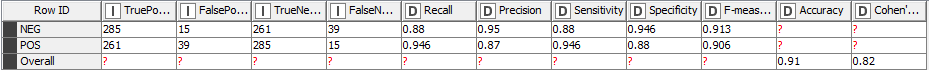
\includegraphics[width=.95\linewidth]{img/classification/scoresRF.png}
    \caption{Medidas estadísticas con Random Forest.}
\end{figure}